% Define document class
\documentclass[twocolumn]{aastex631}
\usepackage{showyourwork}

\usepackage{graphicx}
\usepackage[ruled,vlined,linesnumbered]{algorithm2e}
\usepackage{algorithmic}

\SetKwInput{Parameters}{Parameters}
\SetKwInput{Variables}{Variables}

\usepackage{tabularx,booktabs,multirow,amsmath}
\usepackage{float}
\usepackage[italicdiff]{physics}

\newcommand{\ripple}{\texttt{ripple}}
\newcommand{\python}{\texttt{python}}
\newcommand{\jax}{\texttt{jax}}
\newcommand{\zdethp}{\texttt{zdethp}}
\definecolor{rb4}{HTML}{27408B}
\newcommand{\kw}[1]{{\color{rb4}[KW: #1 ]}}
\definecolor{cyan}{HTML}{0097A7}
\newcommand{\kl}[1]{{\color{cyan}[KL: #1 ]}}
\definecolor{rr}{RGB}{173, 37, 37}
\newcommand{\te}[1]{{\color{rr}[TE: #1 ]}}

\newcommand{\cuhk}{\affiliation{Department of Physics, The Chinese University of Hong Kong, Shatin, N.T., Hong Kong}}
\newcommand{\flatiron}{\affiliation{Center for Computational Astrophysics, Flatiron Institute, New York, NY 10010, USA}}
\newcommand{\JHU}{\affiliation{William H. Miller III Department of Physics and Astronomy, Johns Hopkins University, Baltimore, Maryland 21218, USA}} 

% Begin!
\begin{document}

% Title
\title{Recalibrating Gravitational Wave Phenomenological Waveform Model}

% Author list
\author{Kelvin K.~H.~Lam} 
\email{kelvin33550336@gmail.com}
\cuhk
\author{Kaze W.~K.~Wong} 
\flatiron
\author{Thomas D.~P.~Edwards}
\JHU

\begin{abstract}
    We present a simple and general method of recalibrating gravitational wave
    (GW) phenomenological waveform models jointly. By using {\jax} and
    {\ripple}, we can perform automatic differentiation to functions, which
    allows us to use gradient-based optimization methods to recalibrate waveform
    coefficients in IMRPhenomD model. This method reduces systematic bias
    previously introduced to the model and generally can improve waveform
    accuracy. With recalibrated coefficients, we found that the typical
    \textit{mismatch} has a $50\%$ decrease. Furthermore, we analyze the
    accuracy base on the waveform's intrinsic parameters. We found that waveform
    accuracy has significant dependence on black hole spin. Reduced spin
    approximation introduces degeneracy in spin, which prevented further
    improvement. We isolated regions in the parameter space that does not fit
    the waveform ansatz. These results allow us to understand more about how to
    develop newer phenomenological models. 
\end{abstract}

\section{Introduction} \label{sec:intro}

In the future, the Laser Interferometer Gravitational-wave Observatory (LIGO)
will finish its maintenance and start observing new gravitational wave (GW)
results. This new O4 run is expected to double the rate of current binary black
hole (BBH) observations \citep{abbott2020prospects}. Additionally, the
sensitivity of interferometers will be increased to capture more details of GW.
Having instruments with higher sensitivity, GW models of equal or higher
accuracy than observations should be used to extract GW information. Otherwise,
the extracted information would be affected more by GW models instead of
interferometer sensitivity, resulting in a bottleneck in GW analyses. Although
GW models are accurate enough for current analyses, the accuracy of current
models will no longer suffice for future data analyses
\citep{purrer2020gravitational}. Hence, it is necessary for us to develop and
improve GW models. 

% Waveform families and slight motivation of why we take Phenom model
Currently, three families of GW models are commonly used. They are the
effective-one-body (EOB) \citep{ossokine2020multipolar, cotesta2020frequency, taracchini2014effective}, Numerical Relativity
(NR) surrogate \citep{islam2022surrogate, varma2019surrogate, varma2019surrogate2} and phenomenological (Phenom) models
\citep{husa2016frequency, khan2016frequency, garcia2020multimode, pratten2021computationally}. 
EOB models are constructed by mapping two masses onto an
effective body under an effective metric; NR surrogate models construct
waveforms using combinations of NR waveforms; Phenom models are formulated using
specific ansatz and inspiral approximations. While EOB and NR surrogate models
give better waveform approximants, Phenom waveforms can be produced much faster,
hence it is used mostly in data analysis tasks that requires many waveform
generations. This advantage scales up in data analysis tasks such as matched
filtering and parameter estimation, where many waveforms are required in each
run. This motivates us to improve upon the current framework of Phenom models,
thus can retain the advantage of fast waveform generation while improving the
model's accuracy. 

Automatic differentiation (AD) is a method to calculate derivatives of functions
up to machine precision. In traditional numerical calculations, derivatives are
usually obtained through numerical derivatives. Symbolic derivatives were
available but it was less efficient. Both methods were not viable in machine
learning, where back-propagation requires precise and rapid derivative
calculations. In {\python}, packages including \texttt{pytorch} \citep{pytorch},
\texttt{tensorflow} \citep{tensorflow2015-whitepaper}, etc. utilizes AD to train
machine learning models. AD's algorithm is intuitive in nature. Functions
defined are decomposed into tree structures of primitives, such as addition or
function evaluations. Since these operations are fundamental, they were saved as
pairs internally. Differentiation proceeds forward following the tree structure,
with the application of the chain rule in each step to evaluate its derivative.
Analytic derivatives of such operations are applied in each step and the desired
derivative can then be obtained by composing back the original function
according to the original structure. {\ripple} \citep{ripple} was a new
implementation of IMRPhenomD, one of the models within the Phenom family. It was first implemented
in \texttt{lalsuite} using \texttt{C}. In order to make use of AD, it was
rewritten using \jax, a {\python} package that supports AD. Using
{\ripple}, one can apply AD to GW models to obtain precise derivatives, thus
allowing one to freely use derivative-based algorithms to perform data analyses. 
% Need to cite references for AD

% Put more focus on the joint optimization instead of having a set of more accurate 
% coefficients, since the method is the main point
In this paper, we investigate the possibility of further improving the accuracy
of IMRPhenomD by jointly optimizing all the fitting coefficients given NR
waveforms, and what constraints one may face when trying to further improve. We
find that simply by applying gradient descent algorithm, one can obtain a better
set of waveform coefficients, thus improving the accuracy of the model.
Furthermore, by comparing the accuracy of optimized and original waveforms, we
find that model-generated waveforms are very sensitive to their intrinsic
parameters. Specifically, IMRPhenomD favors certain parts of the parameter
space. This means IMRPhenomD introduces systematic bias to other GW analysis
tasks. This showcases the flaws of the ansatz and allows us to have a deeper
understanding of Phenom models.  

The rest of the paper is structured as follows: In Sec.~\ref{sec:method}, we
review the parameterization of the IMRPhenomD model and the mismatch function
that is used as an objective function for the calibration, followed by outlining the
specific optimization scheme used for recalibration. In
Sec.~\ref{sec:result}, we give the optimization result by comparing mismatches
of optimized waveforms with original waveforms. We also show how the
optimization result differs with waveforms of different intrinsic parameters. In
Sec.~\ref{sec:discussion}, we address the difference between our calibrating
procedure with \citep{khan2016frequency}. We also explain how reduced spin
parameterization affects the accuracy of the model. 

\section{Optimization Method} \label{sec:method}

In this section, we first briefly review the construction of the IMRPhenomD model and discuss
how the calibration parameters enter the waveform.
We then outline the mismatch and how it can be used as a loss fucntion. 
Finally we discuss the gradient descent algorithm and our stopping criterion.

\subsection{Waveform Model} \label{subsec:waveform_model}

% Paragraphs we need:
% 1. What is the model
% 2. How do the parameters enter the model
We start by giving a succinct summary of the IMRPhenomD model and the relevant parameters.
Interested readers should refer to \citep{khan2016frequency} for more details.

Aligned-spin, frequency-domain waveform models (such as IMRPhenomD) can be written as a
combination of amplitude and phase functions ($A$ and $\phi$ respectively):
\begin{align}\label{eq:}
	h(f,\theta,\Lambda) = A(f,\theta,\Lambda)e^{-i\phi(f,\theta,\Lambda)}\,,
\end{align}
where $f$ is the frequnecy, $\theta$ are the intrinsic parameters of the binary, and $\Lambda$ is a set of additional
parameters which will be discussed below. 
The phase and amplitude functions are then split into three sections which represent the
inspiral, intermediate, and merger-ringdown (MR) parts of the waveform. 
During inspiral, $A$ and $\phi$ are known analytically from post-Newtonian (PN) theory;
IMRPhenomD uses the TaylorF2 model \citep{Buonanno:2009zt, Arun:2004hn} which is known up to 3.5PN order.
To model the intermediate and MR regions, IMRPhenomD (and all waveforms in the IMRPhenom family)
uses a series of parameterizations\footnote{
	The parameterizations for both the ampltude and phase functions can be found in \citep{khan2016frequency}.
} 
which depend purely on $\Lambda$ and can be calibrated to numerical relativity (NR) simulations.
The three sections are then \textit{stictched} together using step functions.
Importantly, the parameterizations are chosen such that they can be made $\mathcal{C}^1$ continuous at the
boundary between each section.

In practice the $\Lambda$ parameters are fit for each section independently i.e., intermediate coefficients are fit whilst ignoring the MR region.
Finally, to map the grid of tuned $\Lambda$ parameters back to the intrinsic parameter space, IMRhenomD uses the polynomial function:
\begin{align} \label{eq:Lambda}
	\Lambda^i&=\lambda_{00}^i+\lambda_{10}^i\eta \nonumber \\
	&+(\chi_{\mathrm{PN}}-1)(\lambda_{01}^i+\lambda_{11}^i\eta+\lambda_{21}^i\eta^2) \nonumber \\ 
	&+(\chi_{\mathrm{PN}}-1)^2(\lambda_{02}^i+\lambda_{12}^i\eta+\lambda_{22}^i\eta^2) \nonumber \\
	&+(\chi_{\mathrm{PN}}-1)^3(\lambda_{03}^i+\lambda_{13}^i\eta+\lambda_{23}^i\eta^2)\,,
\end{align}
where the $\lambda$'s are the fitting coefficients we are going to optimize below, $\eta$ is
the symmetric mass ratio, and $\chi_{\mathrm{PN}}$ is the post-Newtonian spin
parameter, which is defined as 
\begin{align}
	\chi_{\mathrm{PN}}=\frac{m_1\chi_1+m_2\chi_2}{m_1+m_2}-\frac{38\eta}{113}(\chi_1+\chi_2)\,.
\end{align}
Here, $m_{1,2}$ and $\chi_{1,2}$ are the primary and secondary mass and spin,
respectively. 

% More precisely, $\Lambda$ by fitting model generated waveforms to Eq.~\ref{eq:amplitude} 
% and the phase ansatzes. Repeating with different NR waveforms, they obtain multiple 
% sets of $\Lambda$, and $\lambda$ are subsequently found by fitting against 
% Eq. \ref{eq:Lambda}. Since the fitting procedure is done in a piece-wise manner, 
% the correlations between different segments are omitted, which could limit the 
% accuracy of the model. Also, since fitting was performed before connecting 
% individual segments, the final waveform does not guarantee to achieve the optimal 
% waveform.
% Finally, the individual segments are first connected directly using 
% step functions. Then, by fixing coefficients in the intermediate segment, one can make 
% the final waveform is continuous in its first derivative.


% In order to recalibrate the model, we have to understand what parameters the model has.
% Here we give a succinct summary of the IMRPhenomD model and the relevant parameters.
% For interested readers, please refer to \citep{khan2016frequency} for more details on construction of the model.

% The IMRPhenomD model is constructed by combining three individually fitted parts
% into one coherent waveform model, which consists of the inspiral, intermediate, and merger-ringdown part, 
% \begin{align}\label{eq:joint_waveform}
% 	h(f,\theta,\Lambda^i)=h_{\mathrm{ins}}(f,\theta,\Lambda^i) + h_{\mathrm{int}}(f,\theta,\Lambda^i) + h_{\mathrm{rd}}(f,\theta,\Lambda^i).
% \end{align}
% Instead of fitting the strain, which is a highly oscillatory function that is
% difficult to fit, the amplitude and phase are fitted since they are smoother
% functions. In each part, the amplitude and phase are made using simple functions
% of frequency such as polynomials or lorentzians. Specifically, the merger-ringdown 
% amplitude is fitted by a lorentzian and the other parts are fitted using polynomials. 
% \begin{equation}\label{eq:amplitude}
% \begin{aligned}
% 	A_0&\equiv\sqrt{\frac{2\eta}{3\pi^{1/3}}}f^{-7/6}\\
% 	A_{\mathrm{ins}}(f;\theta)&=A_{\mathrm{PN}}(f;\theta)+A_0\sum_{i=1}^3\rho_if^{(6+i)/3} \\
% 	A_{\mathrm{int}}(f;\theta)&=A_0(\delta_0+\delta_1f+\delta_2f^2+\delta_3f^3+\delta_4f^4) \\
% 	A_{\mathrm{rd}}(f;\theta)&=A_0\left[\gamma_1\frac{\gamma_3f_{\mathrm{damp}}}{(f-f_{\mathrm{RD}})^2+(\gamma_3f_{\mathrm{damp}})^2}e^{-\frac{\gamma_2(f-f_{\mathrm{RD}})}{\gamma_3f_{\mathrm{damp}}}}\right],  
% \end{aligned}
% \end{equation}
% where $A_{\mathrm{PN}}$ is the post-newtonian expansion of the insprial amplitude up to order $A_0f^2$, $f_{\mathrm{damp}}$ is the damping frequency, and $f_{\mathrm{RD}}$ is the frequency at ringdown. 


%\kw{Need to work on this paragraph}
Although initially independent, the stiching procedure means that each section
of the waveform intrinsically depends on the full set of $\lambda$'s. 
A slightly inaccurate set of $\lambda$'s can therefore lead to inaccuracies in
the generated waveforms. 
Thus, the calibration of these coefficients is crucial to the accuracy
of IMRPhenom GW models. 
Importantly, since the fitting was performed on the individual segments,
the final waveform is not guarenteed to have $\lambda$'s close to global minima.

% Generally, waveform coefficients 
% are obtained by calibrating with NR waveforms, which are waveforms computed 
% using NR simulations. In the case of \citep{khan2016frequency}, they first 
% obtain a set of $\Lambda$ by fitting model generated waveforms to Eq.~\ref{eq:amplitude} 
% and the phase ansatzes. Repeating with different NR waveforms, they obtain multiple 
% sets of $\Lambda$, and $\lambda$ are subsequently found by fitting against 
% Eq. \ref{eq:Lambda}. Since the fitting procedure is done in a piece-wise manner, 
% the correlations between different segments are omitted, which could limit the 
% accuracy of the model. Also, since fitting was performed before connecting 
% individual segments, the final waveform does not guarantee to achieve the optimal 
% waveform. The connecting procedure alters the previously fitted waveform. 
% Hence, the model generated waveforms contains additional inaccuracies. 

At the time of construction this piece-wise approach was necessary since
$\lambda$ has 209 components, making the fitting to NR simulations computationally prohibitive.
Here, for the first time we recalibrate the $\lambda$ coefficients jointly. 
This is made possible by the use of gradient-based optimization algorithms,
enabled by AD from \jax\, and {\ripple}, which are significatnly more efficient in high dimensions.
% , gradients of IMRPhenomD can be easily obtained, thus
% allowing the use of gradient-based algorithms for us to recalibrate the model.   

\subsection{Loss Function} \label{subsec:loss}

In order to optimize the coefficients, we need to define a loss function that
quantifies the difference between waveform model and the target NR simulations which we want to match.
Here we adopt a quantity commonly used in GW physics called the \textit{mismatch} function \citep{husa2016frequency}. 
It is defined as
\begin{align} \label{eq:mismatch}
	\mathcal{M}(h_1, h_2)=1-\max_{t_0, \phi_0}\langle \hat{h}_1, \hat{h}_2\rangle,
\end{align}
where $h_{1,2}$ are the two GW waveforms we are comparing, and $t_0$ and $\phi_0$
are a relative time and phase shift respectively. 
The inner product, $\langle h_1, h_2 \rangle$, is defined as 
\begin{align}\label{eq:inner_prod}
	\langle h_1, h_2 \rangle = 4\Re\int_{f_{\mathrm{min}}}^{f_{\mathrm{max}}}\frac{h_1(f)h_2^{\ast}(f)}{S_n(f)}\,df,
\end{align}
where $\hat{h}=h/\sqrt{\langle h, h \rangle}$ is the normalized GW strain,
$S_n(f)$ is the power spectral density (PSD), $f_{\mathrm{max}}$ and $f_{\mathrm{min}}$ are
the relevant maximum and minimum frequencies for the integration.
We note here that the mismatch can be viewed as the mean square error (MSE) between the
two waveforms.

\te{Up to here}

Since we wish to optimize the model over the whole parameter space, we need to compare multiple model generated waveforms with NR waveforms. However, mismatch only quantifies the difference between IMRPhenomD and NR waveform for one particular set of intrinsic parameters. To take into account of various different waveforms in the parameter space, we pick waveforms from the different parts of the parameter space. We define the loss function as an average of training waveforms in two ways, the simple average of mismatches and the normalize average of mismatches,  
\begin{align}
	\mathcal{L}_{\mathrm{mean}}&=\frac{1}{N}\sum_{i=1}^N\mathcal{M}_i \\
	\mathcal{L}_{\mathrm{fl}}&=\frac{1}{N}\sum_{i=1}^N\frac{\mathcal{M}_i}{\mathcal{M}_{i,\mathrm{ini}}},
\end{align}	
where $\mathcal{M}_i$ represents the mismatch of an individual training waveform,
$\mathcal{M}_{i,\mathrm{ini}}$ represents the initial mismatch of the individual
training waveform, and $N$ is the total number of individual training waveforms.
Note that we choose to use two different averages, since they have different 
preferences in optimization base on waveform mismatches. For the first choice, 
simple average serves as the simplest choice of loss function, but is prone to 
be dominated by a single waveform with a large mismatch. Other waveforms with 
smaller mismatches would be insignificant comparatively, and might not be able 
to improve under such optimization. Alternatively, the second choice, normalized 
average eliminates the aforementioned issue. Nevertheless, it excludes the
information on initial mismatches. $\mathcal{L}_{\mathrm{fl}}$ restricts every
training waveform to decrease at similar rates, hence it is hard to obtain
optimized waveforms with mismatches in the same order of magnitude. Instead,
their ratios in mismatches would remain approximately the same. Conversely,
$\mathcal{L}_{\mathrm{mean}}$ allows the loss function to automatically adjust
and individual mismatches would be in a similar order of magnitude after 
optimization. In this paper, we showcase the results of using both loss functions 
and examine the differences between them. 

\subsection{Optimization Scheme} \label{subsec:optimization}

To compute the loss functions, we have to take NR waveforms for calculating the mismatch. We choose 11-16 NR waveforms from the set of waveforms used in the original
calibration process as training waveforms. Originally, 19 waveforms are taken from 
NR simulations for calibrating IMRPhenomD \citep{khan2016frequency}, 
which are waveforms from the SXS catalog \citep{boyle2019sxs} or BAM simulation. 
As BAM waveforms are not publicly available, we cannot take the identical training 
set as them. Instead, we take the available waveforms from the SXS catalog to construct our loss function. Training waveforms used are listed in Tab.~\ref{tab:q148}~and~\ref{tab:q1248}. The training waveforms chosen has maximum mass ratio to be 8. This is because SXS catalog does not have NR waveforms with extremely high mass ratio. In fact, the SXS catalog only has NR waveforms with $q\leq10$. Nevertheless, we are interested in the behavior of IMRPhenomD model with small $q$, as most BBH events observed from LIGO have $q\leq8$. Hence, we calibrate IMRPhenomD with waveforms of $q\leq8$. 

In the SXS catalog, NR waveforms are in the form of time-series strain. Since time-series data is oscillatory, performing optimization in the time-domain is not ideal. Hence, we transform NR waveforms to frequency-domain to compare with IMRPhenomD waveforms with the
same intrinsic parameters. We taper the time-series using Tukey window.
\footnote{ Specifically, we choose $\alpha=2t_{\mathrm{RD}}/T$, where
	$t_{\mathrm{RD}}$ is the duration of ringdown and $T$ is the duration of the
	entire GW strain. } 
Then, the frequency spectra can be obtained by taking the Fourier transform of the time-series.

%\te{I think this discussion needs to be much more precise. Having a waveform model calibrated to particular noise curve could make sense, but its inherently different to just fitting the phase and the amplitude separately like they do in the original paper. So I would recommend that our default is to use a flat PSD and then in addition discuss the one with the PSD. This way, I think we demonstrate more clearly that its the high dimensional fitting that helps, not the just changing the metric used when fitting.}
Other than NR waveforms, one need to choose a relevant noise PSD for 
mismatch. We have opted to use a flat PSD for this purpose, as it provides results that are independent of the detector sensitivity and mass scale. The use of a flat PSD ensures that the improvement in accuracy is due mainly to the difference in high-dimensional fitting and piece-wise fitting, but not due to the use of a different mass scale. Furthermore, we are interested in examining the effect of introducing a detector PSD on the optimization process. For this, we have chosen the zero-detuned high-power (\zdethp) noise PSD \citep{aasi2015advanced}. Since the total mass of the system scales with the frequency of the waveform, we must choose a corresponding mass scale to match the frequency range of our noise PSD. We selected an arbitrary mass scale of $M=50M_{\odot}$ for all waveforms for demonstration, as this is a commonly observed mass scale in LIGO observations. 
%\te{This choice seems pretty arbitrary. Looking at Fig 8 of 2111.03606, they seem to cluster closer to 60-70. This choice is important and should be more informed.}We will then examine the differences in optimization.

%Other than NR waveforms, one need to choose a relevant noise PSD for 
%mismatch. Since a common goal for creating waveform approximant is to
%deploy the waveform model in downstream data analysis tasks, a reasonable choice
%for the noise PSD should be closely related to the instrument of interest. We
%choose the zero-detuned high-power (\zdethp) noise PSD as our
%first choice of noise PSD \citep{aasi2015advanced}. Because the total mass of the system simple scales
%the frequency of the waveform, we need to choose a corresponding mass scale to
%match the frequency range of our noise PSD. Here, we choose $M=50M_{\odot}$ for
%all waveforms, since this mass scale is common in LIGO observations. In addition
%to a detector-dependent PSD, we are also interested in a more
%instrument-agnostic case such that we can evaluate the effectiveness of the
%recalibration without considering detector effect. In this case, we set the
%noise PSD to be a constant value. 

We point out that our treatment to NR waveforms is different from that of \citep{husa2016frequency, khan2016frequency}. In the original calibration process, training waveforms are hybrid waveforms of NR and SpinAlignedEOB
(SEOB) waveforms. The low frequency inspiral part is taken from the SEOB
waveforms while the rest of the waveforms are taken from NR simulations.
Instead, we solely use NR waveforms for comparison, since we are only exploring the possibility of optimizing waveform models. Thus, for simplicity sake, we ignore this procedure. On the other hand, most NR waveforms used (for both training and testing) have long enough time series data, i.e.~$>15$ orbits \citep{boyle2019sxs}, in
which they are long enough to contain part of the inspiral segment and all
merger and ringdown frequency information. We take the frequency limits as
$f_{\mathrm{min}}=0.1f_{\mathrm{RD}}$ and $f_{\mathrm{max}}=1.2f_{\mathrm{RD}}$,	
where $f_{\mathrm{RD}}$ is the frequency at ringdown. This range covers most of
the IMRPhenomD's frequency range, except the minimum frequency is set higher
than that in the original calibration due to NR length. When compared with
IMRPhenomC, the frequency range is slightly extended to have a higher maximum
frequency. We have the dimensionless frequency spacing $M\Delta f=2.5\times10^{-6}$, 
which is sufficient to capture all features of GW strain. 

With the loss function evaluated, we apply gradient descent to optimize the tunable
coefficients as shown in Algorithm~\ref{alg:gradient}. We take $\lambda_i$ to be the 
original coefficients given in \citep{khan2016frequency}. We take them as the initial 
waveform coefficients because they lie in the neighborhood of the minimum that we wish 
to find. Then, by taking $\alpha=10^{-6}$, we see the validation loss in 
Fig.~\ref{fig:loss} plateau at around $N=12000$, hence we end the optimization here.  
%\te{I think we need a bit more discussion about the stopping criterion here. What is N, and why did we choose it to be this number? Ideally we would actually have a plot of the loss function during training. I don't have a good intuition for if its noisy. Does it plateau? If we wanted to ensure that people don't complain about overfitting we could also plot the loss of the validation set to show its not going up.}

\begin{figure}
	\script{loss.py}
	\centering
	\includegraphics[width=\columnwidth]{figures/loss.pdf}
	\caption{Loss functions against number of iterations. We take the set of coefficients at the minimum of the validation loss.}
	\label{fig:loss}
\end{figure}

\begin{algorithm}[t]
	\caption{Gradient descent pseudocode}
	\label{alg:gradient}
	\KwIn{initial coefficients $\lambda_i$} \Parameters{number of iterations
		$N$, learning rate $\alpha$} \Variables{current coefficients $\lambda$,
		mismatch gradient $\nabla\mathcal{L}$} \KwResult{output coefficients
		$\lambda$} $\lambda\leftarrow\lambda_i$\\
	\tcc{Gradient Descent}
	\For{$i<N$}{ $\mathcal{L}\leftarrow Mismatch(\lambda)$ \\
		$\nabla\mathcal{L}\leftarrow AutoDiff(\mathcal{L})$\\
		$\lambda\leftarrow\lambda-\alpha\nabla\mathcal{L}$\\
	} \Return{$\lambda$}
\end{algorithm}

\begin{figure}[t]
	\script{intrin_space.py}
	\centering
	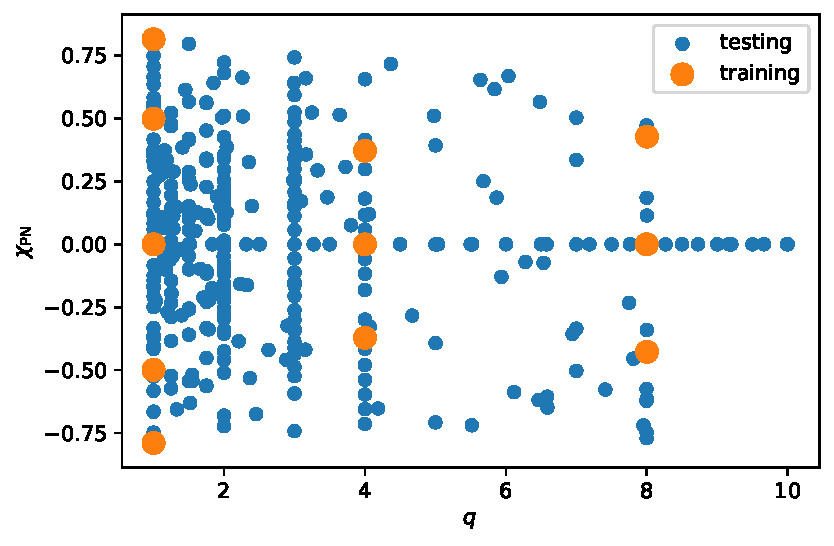
\includegraphics[width=\columnwidth]{figures/intrin_space.pdf}
	\caption{Parameter space with mass ratio $q$ against post-newtonian spin parameter $\chi_{\mathrm{PN}}$. Orange: Training waveforms; Blue: Testing waveforms}
	\label{fig:intrin_space}
\end{figure}

\begin{table}[t]
	\centering
	\begin{tabularx}{0.8\columnwidth}{@{\extracolsep{\fill}}lrrr}
		\toprule\midrule Code         & $q$ & $\chi_1$ & $\chi_2$ \\
		\midrule\midrule SXS:BBH:0156 & 1.0 & -0.95    & -0.95    \\
		SXS:BBH:0151 & 1.0 & -0.60    & -0.60    \\
		SXS:BBH:0001 & 1.0 &  0.00    &  0.00    \\
		SXS:BBH:0152 & 1.0 &  0.60    &  0.60    \\
		SXS:BBH:0172 & 1.0 &  0.98    &  0.98    \\
		SXS:BBH:1418 & 4.0 & -0.40    & -0.50    \\
		SXS:BBH:0167 & 4.0 &  0.00    &  0.00    \\
		SXS:BBH:1417 & 4.0 &  0.40    &  0.50    \\
		SXS:BBH:0064 & 8.0 & -0.50    & -0.46    \\
		SXS:BBH:0063 & 8.0 &  0.00    &  0.00    \\
		SXS:BBH:0065 & 8.0 &  0.50    &  0.46    \\ \midrule\bottomrule
	\end{tabularx}
	\caption{List of waveforms used to recalibrate the model. The mass ratio
	$q=m_1/m_2\geq 1$ with spins $\chi_{1,2}$. Out of the 11 waveforms listed
	here, 9 of them are also used in the original IMRPhenomD calibration.
	\citep{khan2016frequency} The two remaining waveforms were from BAM
	simulation, to which we do not have access.}
	\label{tab:q148}
\end{table}
\begin{table}[t]
	\centering
	\begin{tabularx}{0.8\columnwidth}{@{\extracolsep{\fill}}lrrr}
		\toprule\midrule Code         & $q$ & $\chi_1$ & $\chi_2$ \\
		\midrule\midrule SXS:BBH:0234 & 2.0 & -0.85    & -0.85    \\
		SXS:BBH:0235 & 2.0 & -0.60    & -0.60    \\
		SXS:BBH:0169 & 2.0 & 0.00     & 0.00     \\
		SXS:BBH:0256 & 2.0 & 0.60     & 0.60     \\
		SXS:BBH:0257 & 2.0 & 0.85     & 0.85     \\ \midrule\bottomrule
	\end{tabularx}
	\caption{Additional waveforms used in further recalibration.}
	\label{tab:q1248}
\end{table}

\begin{figure*}[t]
	\script{0154.py}
	\centering
	\includegraphics[width=\textwidth]{figures/0154.pdf}
	\caption{Comparison between original and optimized IMRPhenomD waveforms.
	Here shows the SXS:BBH:0154 NR waveform, which has mass ratio $q=1$ and
	$\chi_1=\chi_2=-0.8$. The original mismatch is around $2.8\times10^{-4}$ and
	the optimized mismatch is around $5.3\times10^{-5}$. Top: It shows the
	amplitude and phase of NR, original IMRPhenomD and optimized IMRPhenomD
	waveform. Bottom: It shows the relative error of amplitudes between NR and
	IMRPhenomD waveforms, and the absolute error of phases between NR and
	IMRPhenomD waveforms}
	\label{fig:0154}
\end{figure*}

\section{Result and Comparison with Original Model} \label{sec:result}

To evaluate the effectiveness of the optimization, we analyze 536 NR waveforms 
from the SXS catalog in this study. We specifically select waveforms with 
negligible eccentricity (${e<2\times10^{-3}}$) and precession 
(${\chi_{x,y}<5\times10^{-3}}$) that are consistent with the constraints of 
the waveform model. As shown in Fig.~\ref{fig:intrin_space}, the intrinsic 
parameters of the chosen test waveforms fall within the parameter space defined 
by the training waveforms. This suggests that these test waveforms can be used 
for direct comparison with the original model.

To illustrate the improvement on an individual waveform level, we compare a
particular waveform before and after optimization in Fig. \ref{fig:0154}.
Compared to the original IMRPhenomD waveform, we can see the optimized waveform
has smaller residual from NR waveform both in amplitude and phase, particularly
in the inspiral region, where the amplitude displays a $50\%$ reduction in
error. For a fair comparison, we selected one of the testing waveforms from the
catalog presented in \citep{khan2016frequency}.

To quantify the effect of optimization over the entire dataset, We evaluate the
mismatch of all testing waveforms using a constant PSD weighted loss function,
$\mathcal{L}_{\mathrm{mean}}$. We present the resulting distribution in Fig.
\ref{fig:q148}. The peak of the distribution has shifted towards a lower
mismatch, with a decrease of almost one order of magnitude and a 50\% reduction
in the median. When using $\mathcal{L}_{\mathrm{fl}}$, we observe a similar
improvement with a 22.9\% decrease in the median. Even though the distribution
lacks a clear peak due to the problem discussed in Section
\ref{subsec:optimization}, both distributions show observable improvement.

\begin{figure}[t]
	\script{q148.py}
	\centering
	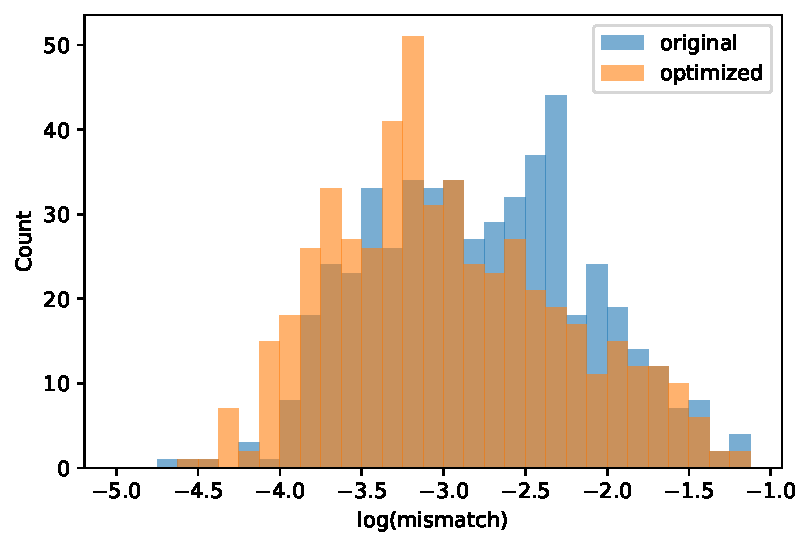
\includegraphics[width=\columnwidth]{figures/q148.pdf}
	\caption{Distributions of waveform mismatches calculated using 
	$\mathcal{L}_{\mathrm{mean}}$. We use training waveforms listed in 
	Tab.~\ref{tab:q148} and	mismatches are weighted with the constant PSD. 
	Dashed lines represent the median of the distributions, which has decreased by 45.3\%.}
	\label{fig:q148}
\end{figure}
\begin{figure}[t]
	\script{q148_q1248_compare.py}
	\centering
	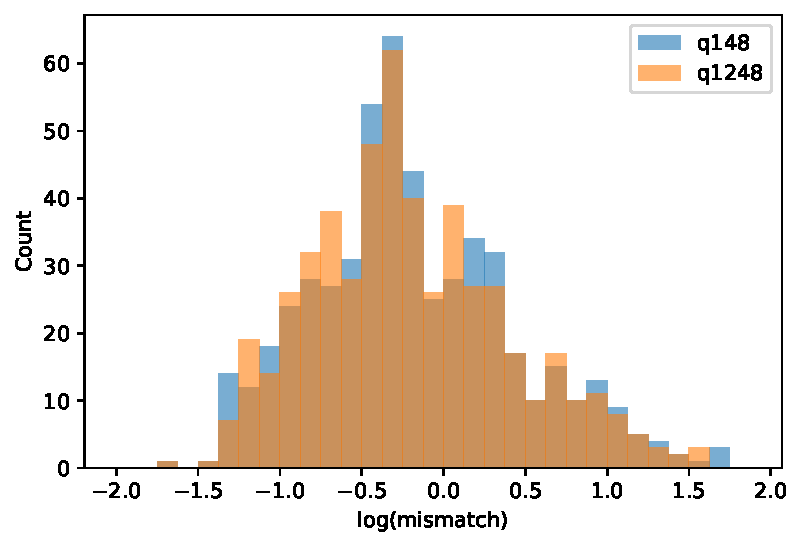
\includegraphics[width=\columnwidth]{figures/q148_q1248_compare.pdf}
	\caption{Distributions of $\log_{10}$ difference in mismatch. The
	distribution labeled \texttt{q148} uses training waveforms listed in
	Tab.~\ref{tab:q148} while the \texttt{q1248} distribution uses waveforms
	listed in Tab.~\ref{tab:q148}~and~\ref{tab:q1248}. Mismatches are calculated
	using the constant PSD with the loss function $\mathcal{L}_{\mathrm{mean}}$. 
	Dashed lines represent the median of the distributions, which has decreased by 10.4\%.}
	\label{fig:q148_q1248_compare}
\end{figure}

%\kw{Which plot is this paragraph referring to?}
Applying the same methods, we will see that the distributions of mismatches
calculated using the {\zdethp} PSD exhibit superior improvement compared to the 
unweighted mismatch.
The shape of the distribution is similar to that shown in Fig. \ref{fig:q148}.
This result is expected, as the IMRPhenomD model was initially constructed and
fitted using the {\zdethp} weighted mismatch. Consequently, the model is
anticipated to closely fit the NR waveforms while incorporating the influence of
the {\zdethp} PSD, rather than a constant PSD.

Motivated by the successful improvement of the waveforms, we expand the training
dataset to optimize additional waveforms listed in Tab. \ref{tab:q1248}. We 
specifically choose to use $q=2$ events since we have abundant $q=2$ NR waveforms 
to validate the final result. The new set of coefficients generated from this
optimization process yields only marginal improvements in the newly produced
waveforms, as seen in Fig. \ref{fig:q148_q1248_compare}. The high mismatch tail
of the optimized distribution remains comparable in length and endpoint to the
original distribution, indicating that our procedure is incapable of improving
these waveforms. Similarly, utilizing the {\zdethp} PSD to optimize the loss
function with additional waveforms leads to similar improvement in the resulting
distribution.

% We believe that either the ansatz does not suit waveforms within certain
% regions of parameter space or the set of optimized coefficients falls to a
% minimum where they do not fit some testing waveforms. If in some region of
% parameter space, the ansatz does not fit well with NR waveforms, it would
% never be able to have consistent improvement under optimization. Instead, it
% would surf around the loss manifold with random fluctuations in mismatches. If
% the set of coefficients does not fit, then dividing the parameter space into
% regions and fitting separate sets of coefficients should give better results.
Although most of the waveforms show improvement in figure \ref{fig:q148}, the
high mismatch tail of the distribution remains unaffected. Given that the
waveform model's ansatz may not be entirely compatible with NR, and the
optimization procedure is carried out over a distribution of waveforms with
varying intrinsic parameters, it is conceivable that some trade-offs in accuracy
exist between different parts of the parameter space. If this is the cause of
the lack of improvement in the high mismatch tail of the distribution,
segmenting the parameter space into smaller subspaces should alleviate this
problem. On the other hand, if the ansatz lacks the correct parameterized form
to capture the NR waveforms' behavior as a function of the intrinsic parameters,
the results will always be biased, and we should not expect any improvement,
even if we segment the parameter space during training.

Since we know intrinsic parameters play an important role in the ansatz, we
would like to investigate how intrinsic parameters affect the recalibration
process. First, we plot the parameter space of $q$ vs. $\chi_{\mathrm{PN}}$ in
Fig. \ref{fig:ps_q148_qchi}. We can see near non-spinning waveforms demonstrate
more consistent improvement, since the ansatz are developed base on non-spinning 
waveforms. Also, the original coefficients were fitted using NR waveforms with
equal or similar spin, hence the model prefers waveforms with similar spin. On 
the other hand, spinning waveforms can either improve or worsen in terms of 
mismatch base on their intrinsic parameters. To further discuss the behavior of 
non-spinning waveforms, we plot the parameter space of $\chi_1$ vs. $\chi_2$ in
Fig.~\ref{fig:ps_q148}. Waveforms along the diagonal axis, i.e. 
$\chi_1\approx\chi_2$, show good mismatch improvements as discussed above. 
Meanwhile, the top-left ($\chi_1<0<\chi_2$) and bottom-right ($\chi_1>0>\chi_2$) 
regions respond to optimization differently. In the top-left 
region, waveforms generally improve slightly with along optimization. However, waveforms 
in the bottom-right region do not improve after optimization. Some waveforms even 
turned worse after optimization. 

\begin{figure}[t]
	\script{ps_q148_qchi.py}
	\centering
	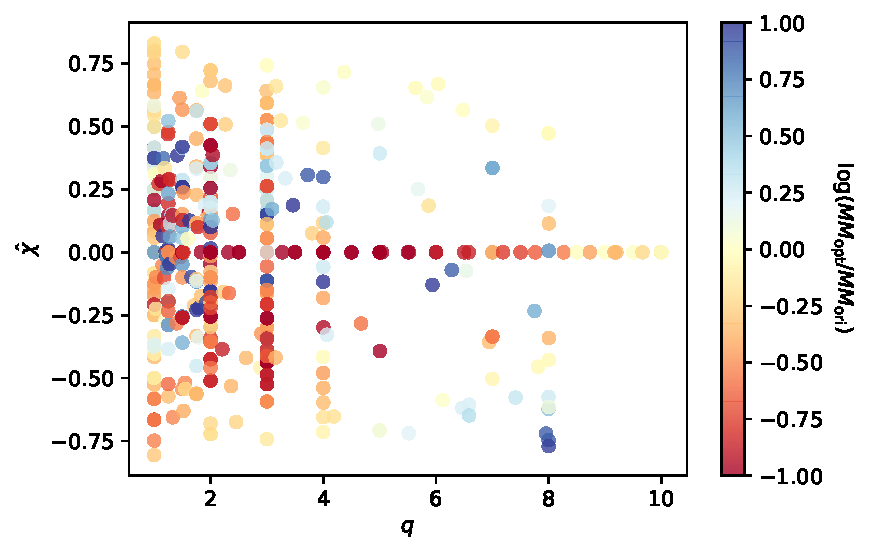
\includegraphics[width=\columnwidth]{figures/ps_q148_qchi.pdf}
	\caption{Parameter space of testing waveforms with $q$ against $\chi_{\mathrm{PN}}$. 
	We show the result from optimizing $\mathcal{L}_{\mathrm{mean}}$ with constant PSD 
	and training waveforms in Tab.~\ref{tab:q148}. Here, the colorbar represents the 
	$\log_{10}$ difference between optimized and original mismatches.}
	\label{fig:ps_q148_qchi}
\end{figure}
\begin{figure}[t]
	\script{ps_q148_chi1chi2.py}
	\centering
	\includegraphics[width=\columnwidth]{figures/ps_q148_chi1chi2.pdf}
	\caption{Parameter space of testing waveforms with $\chi_1$ against $\chi_2$. We
	show the result from optimizing $\mathcal{L}_{\mathrm{mean}}$ with the
	constant PSD and training waveforms listed in Tab.~\ref{tab:q148}.}
	\label{fig:ps_q148}
\end{figure}

\begin{table}[t]
	\centering
	\begin{tabularx}{0.8\columnwidth}{@{\extracolsep{\fill}}lrrr}
		\toprule\midrule Code         & $q$ & $\chi_1$ & $\chi_2$ \\
		\midrule\midrule SXS:BBH:0172 & 1.0 & 0.98     & 0.98     \\
		SXS:BBH:0152 & 1.0 & 0.60     & 0.60     \\
		SXS:BBH:0001 & 1.0 & 0.00     & 0.00     \\
		SXS:BBH:1417 & 4.0 & 0.40     & 0.50     \\
		SXS:BBH:0167 & 4.0 & 0.00     & 0.00     \\
		SXS:BBH:1426 & 8.0 & 0.48     & 0.75     \\
		SXS:BBH:0063 & 8.0 & 0.00     & 0.00     \\ \midrule 
		SXS:BBH:0370 & 1.0 & -0.20    & 0.40     \\
		SXS:BBH:2092 & 1.0 & -0.50    & 0.50     \\
		SXS:BBH:0330 & 1.0 & -0.80    & 0.80     \\
		SXS:BBH:2116 & 2.0 & -0.30    & 0.30     \\
		SXS:BBH:2111 & 2.0 & -0.60    & 0.60     \\
		SXS:BBH:0335 & 2.0 & -0.80    & 0.80     \\
		SXS:BBH:0263 & 3.0 & -0.60    & 0.60     \\
		SXS:BBH:2133 & 3.0 & -0.73    & 0.85     \\
		SXS:BBH:0263 & 4.0 & -0.80    & 0.80     \\ \midrule 
		SXS:BBH:0156 & 1.0 & -0.95    & -0.95    \\
		SXS:BBH:0151 & 1.0 & -0.60    & -0.60    \\
		SXS:BBH:0001 & 1.0 & 0.00     & 0.00     \\
		SXS:BBH:1418 & 4.0 & -0.40    & -0.50    \\
		SXS:BBH:0167 & 4.0 & 0.00     & 0.00     \\
		SXS:BBH:1419 & 8.0 & -0.80    & -0.80    \\
		SXS:BBH:0063 & 8.0 &  0.00    &  0.00    \\ \midrule 
		SXS:BBH:0304 & 1.0 & 0.50     & -0.50    \\
		SXS:BBH:0327 & 1.0 & 0.80     & -0.80    \\
		SXS:BBH:2123 & 2.0 & 0.30     & -0.30    \\
		SXS:BBH:2128 & 2.0 & 0.60     & -0.60    \\
		SXS:BBH:2132 & 2.0 & 0.87     & -0.85    \\
		SXS:BBH:2153 & 3.0 & 0.30     & -0.30    \\
		SXS:BBH:0045 & 3.0 & 0.50     & -0.50    \\
		SXS:BBH:0292 & 3.0 & 0.73     & -0.85    \\ \midrule\bottomrule
	\end{tabularx}
	\caption{List of waveforms used in recalibrating coefficients in 4 regions. From top to down are the top-right ($\chi_1,\chi_2>0$), top-left ($\chi_1<0<\chi_2$), bottom-left ($\chi_1,\chi_2<0$) and bottom-right ($\chi_1>0>\chi_2$) regions. Note that for the top-right and bottom-left regions, waveforms are chosen to have $\chi_1\approx\chi_2$, while the training waveforms for the other two regions are chosen to have $\chi_1\approx-\chi_2$.}
	\label{tab:quadrants}
\end{table}

We divided the parameter space into four regions to analyze the effect of the
recalibration procedure on each region separately (Fig.~\ref{fig:ps_q148_quadrant}). 
The training waveforms used for fitting are listed in Tab.~\ref{tab:quadrants}. The
top-left and bottom-right regions have limited data for $q>4$, hence the results are
only valid up to $q\lesssim4$. From Fig.~\ref{fig:ps_q148_quadrant}, we observe that 
equal-spin waveforms lying on the diagonal has great improvement. Above the diagonal, 
the improvement is significant, except for a few defects caused by some testing waveforms 
having $q>4$. This can be seen clearer in Fig.~\ref{fig:all_quadrants}, which we see 
that the optimized histogram shifts downward uniformly. Below the diagonal, waveforms 
have negligible improvement (Fig.~\ref{fig:all_quadrants}~and~\ref{fig:ps_q148_quadrant}), 
indicating the original set of coefficients is the optimal set of coefficients, and 
cannot be further improved. Hence, we can deduce IMRPhenomD has better match with the 
top-left region and does not fit well with waveforms lying in the bottom-right 
region. Thus, the ansatz restricts additional improvements and further optimizing in a 
smaller region does not generally improve the results.

\begin{figure}[t]
	\script{all_quadrants.py}
	\centering
	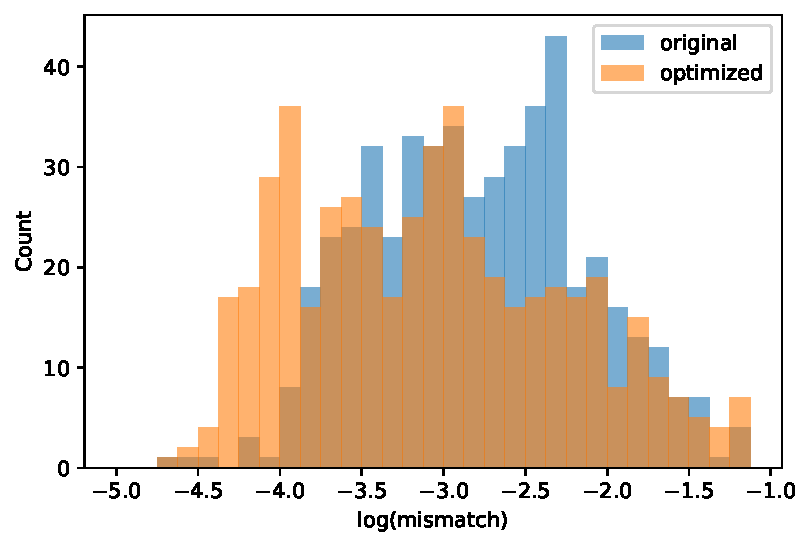
\includegraphics[width=\columnwidth]{figures/all_quadrants.pdf}
	\caption{Distributions of mismatches in the top-left (Top) and bottom-right (Bottom) regions.
	We use a constant noise spectrum to calculate mismatch and
	$\mathcal{L}_{\mathrm{mean}}$ as the loss function. Waveforms in the top-left region generally improves while waveforms in the bottom-right region has very little improvement, as indicated by the median (dashed lines).}
	\label{fig:all_quadrants}
\end{figure}

\begin{figure}[t]
	\script{ps_q148_quadrants.py}
	\centering
	\includegraphics[width=\columnwidth]{figures/ps_q148_quadrants.pdf}
	\caption{Parameter space of testing waveforms. Each region is fitted independently with waveforms listed in Tab.~\ref{tab:quadrants}.}
	\label{fig:ps_q148_quadrant}
\end{figure}

\section{Discussion} \label{sec:discussion}

We have shown the result of recalibrating waveform coefficients. One thing to
note is that our recalibration procedure is not exactly the same as the original
calibration. For instance, we use a different set of NR waveforms, frequency
range, etc. Nonetheless, as the decrease in mismatch is rather significant, this
optimization procedure should be able to improve the accuracy of IMRPhenomD on a
similar scale regardless of the differences. Here, the result serves as a
demonstration of the general method used.  

The results presented in Fig.~\ref{fig:q148_q1248_compare} demonstrate that
increasing the number of training waveforms used in waveform optimization yields
only a marginal increase in accuracy. Our analysis suggests that this marginal
improvement is a consequence of over-determination of the waveform coefficients.
Consequently, increasing the number of calibration NR waveforms is unlikely to
result in any significant improvement of the model's accuracy. These
observations suggest that the parameterized ansatz employed in our study may not
be suitable for certain regions in the parameter space, leading to low mismatches
for some waveforms while other waveforms remain at the high mismatch tail with
negligible changes. This highlights the constraints of the model's flexibility
that ultimately limit its performance.

The reduced spin approximation is a major contributor to the inaccuracies
observed in the ansatz. In IMRPhenomD, this approximation employs a single spin
parameter, $\chi_{\mathrm{PN}}$, as described in Sec.~\ref{sec:method}. The
parameterization of BBH mergers using a single spin parameter results in a
degeneracy within the parameter space. Specifically, black hole events with
different spins may generate the same waveform due to identical values of
$\chi_{\mathrm{PN}}$, leading to erroneous results, particularly for highly
unequal spin events. This degeneracy produces straight lines in the parameter
space with negative slopes that depend on the mass ratio, which can be seen in 
Fig.~\ref{fig:ps_q148}. Notably, the ansatz performs better in the top-left
region than the bottom-right region. In an attempt to address
this issue, we partitioned the parameter space into four regions, as described
in Sec.~\ref{sec:result}. With separate optimizations for each
regions, Fig.~\ref{fig:ps_q148_quadrant} indicates that the top-left region's 
performance has improved, while the bottom-right region hardly improves. 
This observation suggests the ansatz is specific to certain regions of the 
parameter space, with a preference for BBH events lying above the diagonal, 
and it has limited enhancement for events lying below the diagonal. 

The division of the parameter space into four regions was a simple approach
taken for practical reasons. A more systematic approach would involve the use of
level set estimation algorithms to identify regions of interest within the
parameter space. Such an algorithm can reveal additional degeneracies or issues
that may exist within the ansatz. One possible strategy is to recalibrate
individual regions of interest to achieve better results. An alternative
approach is to select regions based on degeneracy lines. However, due to the
limited number of NR waveforms available, we were unable to implement this
approach. With more NR waveforms available in the future that cover the entire
parameter space, we can perform optimization with fewer restrictions and select
regions more systematically. Other than how to divide regions of interest, the 
choice of training waveforms also affects the final results greatly. Note that 
the choice of training waveforms listed in Tab.~\ref{tab:quadrants} were taken 
arbitrarily to test the effectiveness of separate fitting. Hence, if one takes 
a different set of training waveforms over the parameter space, the result might 
give additional features that can test and explain IMRPhenomD better. 

Although our study primarily focused on the IMRPhenomD model, this simple yet
versatile approach can be applied to other differentiable GW models, such as the
IMRPhenomP \citep{hannam2014simple, khan2019phenomenological} or IMRPhenomX \citep{pratten2020setting,pratten2021computationally} 
models within the same family. By jointly optimizing a new set of coefficients,
it is expected that both models can be enhanced since they share similar
construction principles to the IMRPhenomD model. For instance, they also use PN
approximants as part of the ansatz in the inspiral segment. It will be interesting 
to recalibratethe IMRPhenomXAS model \citep{pratten2020setting}. Because it is
parameterized by an additional anti-symmetric spin parameter, it is expected not
to exhibit the degeneracy previously described. With the currently developing 
{\jax} IMRPhenomXAS model in {\ripple}, A more detailed investigation
may provide valuable insights into the systematics of the Phenom models.
Furthermore, this approach is applicable to other GW model families, such as NR
surrogate models or EOB models introduced in Sec. \ref{sec:intro}. Such an approach could 
simplify NR waveform calibration procedures and lead to the improvement of 
existing models.

\section{Conclusion} \label{sec:conclusion}

In this paper, we have presented a systematic method to recalibrate GW models.
This method utilizes {\jax}'s automatic differentiation to apply
derivative-based optimization to recalibrate GW models jointly. Using the new
implementation of the IMRPhenomD model, {\ripple}, which is written in \jax, in
conjunction with NR waveforms from the SXS catalog, we recalibrate waveform
coefficients of the IMRPhenomD model. In general, the waveform accuracy can be
improved by 50\%. Comparing {\zdethp} weighted and unweighted mismatch, weighted
mismatches have a slightly better improvement. In contrast, different types of
loss function result in significantly different final mismatch distributions. As 
seen in Fig.~\ref{fig:q148}, $\mathcal{L}_{\mathrm{mean}}$ outperforms 
$\mathcal{L}_{\mathrm{fl}}$. By increasing the number of training waveforms, we see a 
slight improvement increase in Fig.~\ref{fig:q148_q1248_compare}. 

Furthermore, we investigated how the intrinsic parameters affect the
improvement. Fig.~\ref{fig:ps_q148} shows that the optimization procedure has a
certain preference for waveforms lying in the top-left region while the bottom-right 
region hardly improved. To further test this result, we recalibrate
waveforms in separate regions in parameter space. From Fig.~\ref{fig:ps_q148_quadrant}, 
we can see that this recalibration process gives further
improvement to the top-left region while the bottom-right region only have little 
improvement. This indicates that the ansatz has limited match in this region and 
does not fit most waveforms in this region, hence introduces bias to downstream GW 
analysis. This phenomenon is mainly due to the reduced spin approximation used in 
parameterizing the ansatz, where degeneracies between $\chi_1$ and $\chi_2$ are introduced. 

While we naively separate the optimization process into 4 regions, one can
perform systematic region-selection. In principle, we can apply this general
method to other newer and more accurate models such as IMRPhenomX or IMRPhenomP
models. Then, we can perform all the above analyses to understand how to
construct better GW Phenom models in the future.  

\section{ACKNOWLEDGMENTS}

We thank Will M.~Farr, Max Isi, and Mark Hannam for helpful discussions; we also
thank Carl-Johan Haster, Neil J.~Cornish and Thomas Dent for comments on the
draft. The Flatiron Institute is a division of the Simons Foundation. T.E.\ is
supported by the Horizon Postdoctoral Fellowship.
\bibliography{bib}

\end{document}
